\documentclass[a4paper, 14pt]{extarticle}
\usepackage[T1,T2A]{fontenc}
\usepackage[utf8]{inputenc}
\usepackage[english,ukrainian]{babel}
\usepackage{amsmath, amssymb, amsthm, mathtools}
\usepackage{bbm}
\usepackage{tikz}
\usetikzlibrary{positioning}
\usepackage{cancel}
\usepackage{graphicx}
\usepackage{color} 
\usepackage{hyperref}
\usepackage{xcolor}
\hypersetup{
    colorlinks=true, %set true if you want colored links
    linktoc=all,     %set to all if you want both sections and subsections linked
    linkcolor=blue,  %choose some color if you want links to stand out
}
\usepackage{geometry}
 \geometry{
 a4paper,
 total={170mm,257mm},
 left=10mm,
 top=10mm,
 right=10mm
 }
\begin{document}

\begin{center}
    \topskip0pt
    \vspace*{\fill}
    \textsc{{Звіт}}\\
    \textsc{до лабораторної роботи №1}\\
    \textsc{{з проблем багатозначного аналізу}}\\
    \textsc{}\\
    \vspace*{\fill}
    \textsc{{Київ, 2021}}\\
    \textsc{{Живолович Олександра}}
\end{center}
\thispagestyle{empty}

\newpage
\thispagestyle{empty}
\tableofcontents

\section{Постановка задачі}
Побудувати графік субдиференціалу функції 
\begin{equation}
f(x_1,x_2) = |-4x_1+2x_2+4| + |2x_1+3x_2-2| + 0.1(x_1-3x_2)^6, \quad (x_1,x_2) \in \mathbb{R}^2.
\end{equation}
Розв'язати задачу 
\begin{equation}
    f(x_1,x_2) \to\min
\end{equation}
\section{Алгоритм}
Нехай $f:\mathbb{R}^n\to\mathbb{R}$ опукла. Для мініміщації $f$,
використовуємо субградієнтний метод
\begin{equation}
    x_{k+1} = x_k - \alpha_k g(x_k)
\end{equation} 
де $x_k$ є $k$-тою точкою ітерації, $g(x_k)$ - будь-який субградієнт 
функції $f$ у точці $x_k$, $\alpha_k$ - розмір $k$-того кроку.

Отже, на кожному році методу, ми робимо крок у напрямку 
від'ємного субградієнту функції $f$. У точках, де 
$f$ диференційовна, субградієнт співпадає з градієнтом функції, а отже 
у цих точках метод зводиться до градієнтного методу.

Оскільки метод не є методом спуску, то гарним підходом 
є збереження найкращого поточного результату 
\begin{equation*}
    f^{(k)}_{\text{best}} = \min\{f^{(k-1)}_{\text{best}}, f^{(k)}\}
    \implies f^{(k)}_{\text{best}} =
    \min\{f(x_1),\hdots , f(x_k)\}.
\end{equation*}

Важливою частною методу є спосіб вибору $\alpha_k$ - розміру кроку.
Існують наступні широковживанні методи вибору $\alpha_k$:
\begin{itemize}
    \item Метод постійного розміру кроку
    \[
    \alpha_k = h    
    \]
    \item Метод кроку постійної довжини
    \[
    \alpha_k = \frac{h}{||g(x_k)||}    
    \]
    \item Метод сумовних з квадратом кроків
    \[
    \sum_{k=1}^\infty \alpha_k^2 <\infty, \quad 
    \sum_{k=1}^\infty \alpha_k = \infty
    \]
    Наприклад, $\alpha_k = a/(b+k), \, a>0,\,b\geq0$.
    \item Метод несумовних кроків, що зменшуються
    \[
        \lim_{k\to\infty}\alpha_k = 0,
        \quad\sum_{k=1}^\infty \alpha_k = \infty  
    \]
    Наприклад, $\alpha_k = a/\sqrt{k}$.
\end{itemize}
\section{Код}
Було обрано мову програмування \emph{Python3}, оскільки 
вона є дуже зручною для роботи з науковими обчисленнями,
а також існують багато зручних пакетів для візуалізації даних.
Код можна знайти за \href{http://www.example.com}{посиланням}.
\section{Висновки}
Була вирішена задача негладкої оптимізації за допомогою субградієнтного
методу. Були зроблені такі спостереження:
\begin{enumerate}
    \item Оскільки функція дуже швидко зростає, то 
    потрібно відразу брати малі кроки для того щоб метод був збіжний
    \item Надто малий розмір року призводить до вкрай повільної збіжності
    \item Методи постійного розміру кроку та 
    постійної довжини кроку показують гарні результати, але потребують 
    гарного підбору параметру.
    \item Метод сумовних з квадратом крокыв показав гарний результат 
    тыльки в одному випадку, але можливо треба просто вдало підібрати параметр.
    \item Метод несумовних кроків, що зменшуються показав 
    дуже гарний результат, але треба розуміти що зменшувати розмір 
    параметру потрібно обережно, адже можно швидко 
    прийти до дуже повільної збіжності. 
\end{enumerate}
\newpage
\begin{thebibliography}{1}
\bibitem{1}
\emph{Subgradient Methods},
Stephen Boyd, Lin Xiao, and Almir Mutapcic
Notes for EE392o, Stanford University, Autumn, 2003
\end{thebibliography}
\newpage
\section{Додатки}
\begin{figure}[h]
    \centering
    \caption{Постійний розмір кроку}
    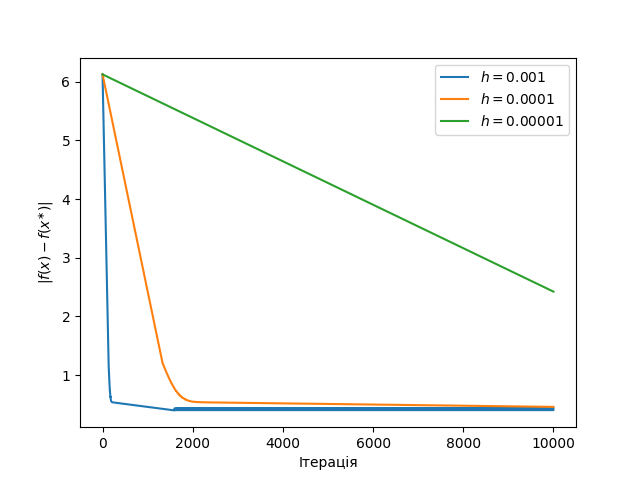
\includegraphics{const_size.png}
\end{figure}
\begin{figure}[h]
    \centering
    \caption{Постійна довжина кроку}
    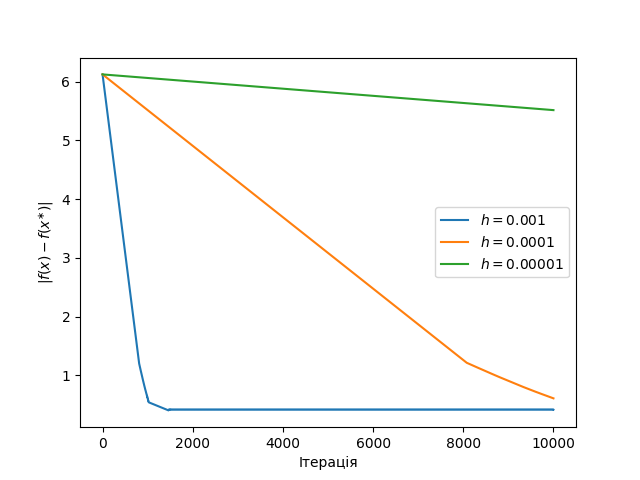
\includegraphics{const_len.png}
\end{figure}
\begin{figure}[h]
    \centering
    \caption{Сумовні з квадратом кроки}
    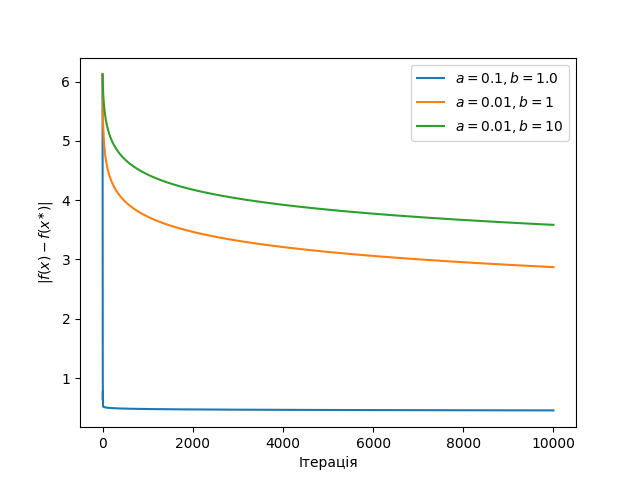
\includegraphics{square_summable.png}
\end{figure}
\begin{figure}[h]
    \centering
    \caption{Кроки, що зменшуються}
    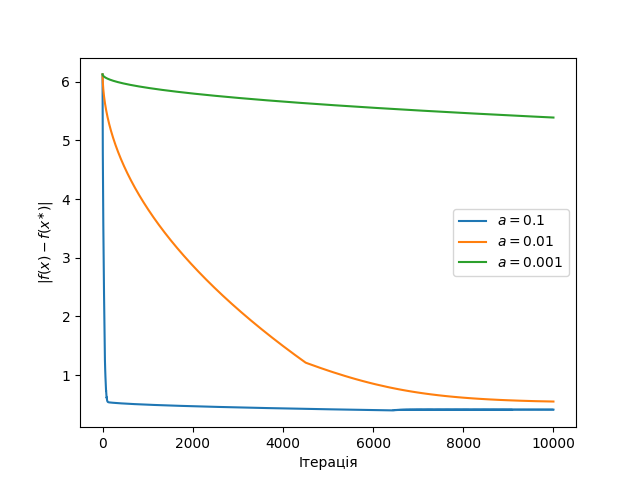
\includegraphics{diminishing.png}
\end{figure}
\end{document}